%% ****** Start of file apstemplate.tex ****** %
%%
%%
%%   This file is part of the APS files in the REVTeX 4 distribution.
%%   Version 4.1r of REVTeX, August 2010
%%
%%
%%   Copyright (c) 2001, 2009, 2010 The American Physical Society.
%%
%%   See the REVTeX 4 README file for restrictions and more information.
%%
%
% This is a template for producing manuscripts for use with REVTEX 4.0
% Copy this file to another name and then work on that file.
% That way, you always have this original template file to use.
%
% Group addresses by affiliation; use superscriptaddress for long
% author lists, or if there are many overlapping affiliations.
% For Phys. Rev. appearance, change preprint to twocolumn.
% Choose pra, prb, prc, prd, pre, prl, prstab, prstper, or rmp for journal
%  Add 'draft' option to mark overfull boxes with black boxes
%  Add 'showpacs' option to make PACS codes appear
%  Add 'showkeys' option to make keywords appear
%\documentclass[aps,prl,preprint,groupedaddress]{revtex4-1}
%\documentclass[aps,prl,preprint,superscriptaddress]{revtex4-1}
\documentclass[aps,prl,reprint,groupedaddress]{revtex4-1}

\usepackage{multirow}
\usepackage{graphicx}% Include figure files
\usepackage{dcolumn}% Align table columns on decimal point
\usepackage{bm}% bold math
\usepackage{longtable}
\usepackage{afterpage}
\usepackage{tabularx}
\usepackage{upquote}
\usepackage{listings}
\usepackage[version=3]{mhchem}
\usepackage[]{SIunits}
\usepackage{multirow}

% You should use BibTeX and apsrev.bst for references
% Choosing a journal automatically selects the correct APS
% BibTeX style file (bst file), so only uncomment the line
% below if necessary.
%\bibliographystyle{apsrev4-1}

\begin{document}

% Use the \preprint command to place your local institutional report
% number in the upper righthand corner of the title page in preprint mode.
% Multiple \preprint commands are allowed.
% Use the 'preprintnumbers' class option to override journal defaults
% to display numbers if necessary
%\preprint{}

%Title of paper
\title{A Exam: Pair Product Projector}

% repeat the \author .. \affiliation  etc. as needed
% \email, \thanks, \homepage, \altaffiliation all apply to the current
% author. Explanatory text should go in the []'s, actual e-mail
% address or url should go in the {}'s for \email and \homepage.
% Please use the appropriate macro foreach each type of information

% \affiliation command applies to all authors since the last
% \affiliation command. The \affiliation command should follow the
% other information
% \affiliation can be followed by \email, \homepage, \thanks as well.
\author{Junhao Li}
\email[]{jl2922@cornell.edu}
%\homepage[]{Your web page}
%\thanks{}
%\altaffiliation{}
\affiliation{
Department of Physics and Laboratory of Atomic and Solid State Physics\\
Cornell University, Ithaca, NY 14853, USA
}

%Collaboration name if desired (requires use of superscriptaddress
%option in \documentclass). \noaffiliation is required (may also be
%used with the \author command).
%\collaboration can be followed by \email, \homepage, \thanks as well.
%\collaboration{}
%\noaffiliation

\date{\today}

\begin{abstract}
% insert abstract here
\end{abstract}

% insert suggested PACS numbers in braces on next line
\pacs{}
% insert suggested keywords - APS authors don't need to do this
%\keywords{}

%\maketitle must follow title, authors, abstract, \pacs, and \keywords
\maketitle

% body of paper here - Use proper section commands
% References should be done using the \cite, \ref, and \label commands
% Put \label in argument of \section for cross-referencing
\section{\label{sec:background}Background}
Quantum Monte Carlo (QMC) method is capable of solving the Schrödinger equation with high accuracy while scales nicely as a function of system size.
The accuracy comes from the insistence of using the 3N-dimensional many-electron wave function as the basic quantity, as apposed to subsumming the complexity into lower-dimentional functions, such as the exchange-correlation functional in DFT.
In addition, we can use pseudopotentials to reduce the number of dimensions and incorporate relativistic corrections.
And QMC, while trying to keep the exact valence-valence correlation, can also give better estimation of the core-valence correlation than mean-field based methods.

A typical QMC calculation of the ground-state energy $E_0$ proceeds as follows. First we come up with a trial wave function $\Psi_T$ with tunable parameters.
We optimize these parameters with variational Monte Carlo (VMC).
Then we try to sample $f = \Psi_0\Psi_T$ and calculate the local energy $E_L = H\Psi_T/\Psi_T$.
Here $\Psi_0$ is the exact ground-state wave function.
And finally the ground-state energy is given by the average local energy
\begin{equation}
E_0 = \frac{\langle \Psi_0|H|\Psi_T \rangle}{\langle \Psi_0|\Psi_T \rangle}
= \frac{\int f(\mathbf{R})E_L(\mathbf{R})d\mathbf{R}}{\int f(\mathbf{R})d\mathbf{R}} \approx \langle E_L \rangle
\end{equation}

To sample $f = \Psi_0\Psi_T$, the traditional approach is through diffusion Monte Carlo (DMC) with fixed-node approximation (FN).

DMC starts from an initial guess $f = \Psi\Psi_T$ and propagates $\Psi$ in imaginary time $\tau=it$.
Suppose the expansion of $\Psi$ in terms of the eigenfunctions of the Hamiltonian is
\begin{equation}
\Psi = \sum_{n=0}^{\infty}c_n\phi_ne^{-(E_n-E_T)\tau}
\end{equation}
We can see that as $\tau\to\infty$, all the excited-state eigenfunctions die away, and through carefull control of $E_T$, we will have $\Psi\to\phi_0=\Psi_0$ and $f\to\Psi_0\Psi_T$.
In practice, we represent $f$ with an ensemble of walkers with attached weights in the 3N-dimentional space.
According to the Schrödinger equation, $\Psi$ evolves in imaginary time as
\begin{equation}
\label{eq:img_sho}
-\frac{\partial \Psi}{\partial \tau} = -\frac{1}{2}\nabla^2\Psi+(V-E_T)\Psi
\end{equation}
%
% \begin{equation}
% \label{eq:G1}
% G_1(\bm{R'}|\bm{R};\tau)
% = \frac{1}{(2\pi\tau)^{3N/2}} e^{-\frac{(\bm{R'}-\bm{R})^2}{2\tau}} e^{-\left(V-E_T\right)\tau}
% \end{equation}
% Here $V = (V(\bm{R'})+V(\bm{R}))/2$.
substituting $f=\Psi\Psi_T$ into Eq.~(\ref{eq:img_sho}) and rearrange, we get $f$ envolves as
\begin{equation}
\label{eq:f}
-\frac{\partial f}{\partial \tau} = -\frac{1}{2}\nabla^2f+\nabla\cdot(v_Df)+(E_L-E_T)f
\end{equation}
where $v_D = \nabla\Psi/\Psi$.
The right hand side of Eq.~(\ref{eq:f}) can be viewed as a diffusion term $-\frac{1}{2}\nabla^2f$, a drifting term $\nabla\cdot(v_Df)$, and a reweighting term $(V-E_T)f$.
In short-time approximation, we can treat each separately, adjust the positions of the walkers according to the diffusion term and the drifting term, and weights according to the reweighting term.
This process can be represented by a probability transition matrix, or a projector
\begin{equation}
\label{eq:G1t}
\widetilde{G}_1(\bm{R'}|\bm{R};\tau)
= \frac{1}{(2\pi\tau)^{3N/2}} e^{-\frac{(\bm{R'}-\bm{R}-\bm{v}(\bm{R})\tau)^2}{2\tau}} e^{-\left(E_L-E_T\right)\tau}
\end{equation}
Here $\bm{v}(\bm{R}) = \nabla\Psi(\bm{R})/\Psi(\bm{R})$ and $E_L = (E_L(\bm{R'})+E_L(\bm{R}))/2$.
After a reasonable amount of steps, the distribution and the weights of the walkers resemble $f=\Psi_0\Psi_T$.

This pure DMC works well for single-particle systems.
However, when dealing with many-electron systems, it suffers from the well-know ``fermion sign problems''.
In the setting mentioned above (1st-quantized basis), this problem has two main components.
First, the dominant state is a bosonic state, instead of a fermionic state.
Second, weights can become negative and walkers representing $\Psi_0$ and $-\Psi_0$ will build up. Since they are equally good wave functions, a severe signal-to-noise issue will occur.

Fixed-node approaximation avoids this problem by forcing the walkers to stay within their initial nodal pockets of $\Psi_T$, thus the signs of the walkers remain unchanged.
It produces the exact ground-state energy if the nodes of the trail function coincide with the exact ones.
Otherwise, the variational principle applies and we will get a slightly higher energy.

Several ways of optimizing the behavior near the nodal surfaces are being actively developed, such as release-node method and stochastic reconfiguration.

\section{Pair Product Projector}

Fixed-node approximation solves the ``fermion sign problems'' at the cost of forcing wave functions to have certain nodes at certain places, which according to the variational principle will give a systematically higher grond state energy.
Methods trying to improve upon this can ameliorate the bias but still cannot get away from it.
Therefore, we seek to approach from a new direction: instead of forcing the wave function to have certain nodal surfaces in order to get the higher fermionic state, we build the antisymmetrization of the wave function into the projector, so its intrinsic ground state would be the fermionic state, which is exactly the state we need for electrons.

We achieve this by summing the contribution to all the permutations of $\bm{R'}$:
\begin{equation}
\label{eq:ppp}
\widetilde{G}_2(\bm{R'}, \bm{R},\tau)
= \sum\limits_{\sigma\in P} \mathrm{sgn}(\sigma) \widetilde{G}_1(\sigma(\bm{R'}), \bm{R}, \tau)
\end{equation}
Here $P$ is the set of all the permutations of the set $\{x:x \in I, 1 \leq x \leq N\}$, $N$ is the number of electrons.
$\mathrm{sgn}(\sigma)$ means the sign of a permutation, which equals to $+1$ if $\sigma$ is even and $-1$ if $\sigma$ is odd.
$\widetilde{G}_1$ is the usual projector, which does not take into account the antisymmetricity of the wave function of the identical fermions.

$\widetilde{G}_1$ can either be the one from DMC as shown in Eq.~(\ref{eq:G1t}), or can be constructed using the pair actions from the path integral Monte Carlo (PIMC).

When using the first approach, we need to use a nodeless guiding wave function $\Psi_G$ for $\Psi_T$ in $f$, otherwise, we are still imposing the fixed-node assumption, because the drifting term forbids the crossing of nodal surfaces.
In doing so we will face a dilemma:
One one hand, we want $\Psi_G$ to be as close to $|\Psi_T|$ as possible, so that the fluctuation in $E_L$ will become smaller and we will achieve a smaller uncertainty quicker.
On the other hand, we have to smooth $|\Psi_T|$ near the nodal surfaces, and we wish the smooth area to be large so that the second derivative near the nodal surfaces can be smaller, which makes the walkers more stable.

The rest of this report will be focusing on the second approach, which starts from pair actions.
In this approach, we use
\begin{align}
\label{eq:G1ppp}
\widetilde{G}_1 = \Psi_G(\bm{R'})G_1(\bm{R'}|\bm{R};\tau)/\Psi_G(\bm{R})\\
G_1 =
\prod\limits_{\alpha = 1}^{N_{\mathrm{nuc}}}\prod\limits_{i=1}^{N}
p_{en}(\bm{r}_i'-\bm{r}_\alpha|\bm{r}_i-\bm{r}_\alpha;\tau)\\
\prod\limits_{1\leq i < j \leq N}p_{ee}(\bm{r}_j'-\bm{r}_i'|\bm{r}_j-\bm{r}_i;\tau)
e^{E_T}
\end{align}
Where $p_{en}$ and $p_{ee}$ are the pair projectors representing electron-nuclei and electron-electron interactions respectively.
They are the inverse of the pair action from PIMC.
One advantage of starting from the pair actions is that, with the same $\tau$, the time step error in this approach shall be smaller than the first approach, because the pair actions are calculated with much smaller time steps.

One method of obtaining the pair action is matrix squaring.
It starts from an extremely small $d\tau = \tau/2^n$, obtain its pair action, and squaring this action to get the value corresponding to the $\tau$ we want.
Here $n$ is some large positive integer.
As $d\tau \to 0$, we can approximate the path with a straight line and obtain its action.

The disadvange is that there will be an electron-electron action term, which forbids us from packing all the terms into a determinant and evaluate in $O(n^3)$ time.
In other words, the computational cost of obtaining the exact pair product projector as shown in Eq.~(\ref{eq:ppp}) is $O(n!)$.
There maybe some algorithm capable of solving this in polynomial time.
The equivalent form of this problem is:
Suppose $M$ is a matrix of dimention $N^4$.
Is there a polynomial time algorithm for calculating
\begin{equation}
\label{eq:algo}
\sum\limits_{\sigma \in P}\prod\limits_{1\leq i < j \leq N}\mathrm{sgn}(\sigma)M_{i,j,\sigma(i),\sigma(j)}
\end{equation}
Here same as before, $P$ is the set of all the permutations.
Although we have not found a polynomial time algorithm yet, there are some approximation algorithms that give results close to the exact sum.

\section{Approximations}

One approach to get an approximated sum is packing all the electron-nuclei actions into a determinant, which can be evaluated in $O(n^2)$, and use an average $U_{ee}$ for the electron-electron interaction.
For example, we can use the following two approximated $U_{ee}$.
\begin{center}
\begin{eqnarray}
U_{ee} = \sum\limits_{i<j}
\frac{u_{ee}(\bm{r}_{ij}'|\bm{r}_{ij}';\tau) + u_{ee}(\bm{r}_{ij}|\bm{r}_{ij};\tau)}{2}\\
U_{ee} = \sum\limits_{i<j}u_{ee}(\bm{r}_{ij}'|\bm{r}_{ij};\tau)
\end{eqnarray}
\end{center}
Here $u_{ee}$ are the pair action.
So the overall $G_2$ becomes
\begin{equation}
\label{eq:G2pppUee}
G_2(\bm{R'}|\bm{R};\tau) =
\end{equation}

\subsection{}
\subsubsection{}

% If in two-column mode, this environment will change to single-column
% format so that long equations can be displayed. Use
% sparingly.
%\begin{widetext}
% put long equation here
%\end{widetext}

% figures should be put into the text as floats.
% Use the graphics or graphicx packages (distributed with LaTeX2e)
% and the \includegraphics macro defined in those packages.
% See the LaTeX Graphics Companion by Michel Goosens, Sebastian Rahtz,
% and Frank Mittelbach for instance.
%
% Here is an example of the general form of a figure:
% Fill in the caption in the braces of the \caption{} command. Put the label
% that you will use with \ref{} command in the braces of the \label{} command.
% Use the figure* environment if the figure should span across the
% entire page. There is no need to do explicit centering.

\begin{figure}
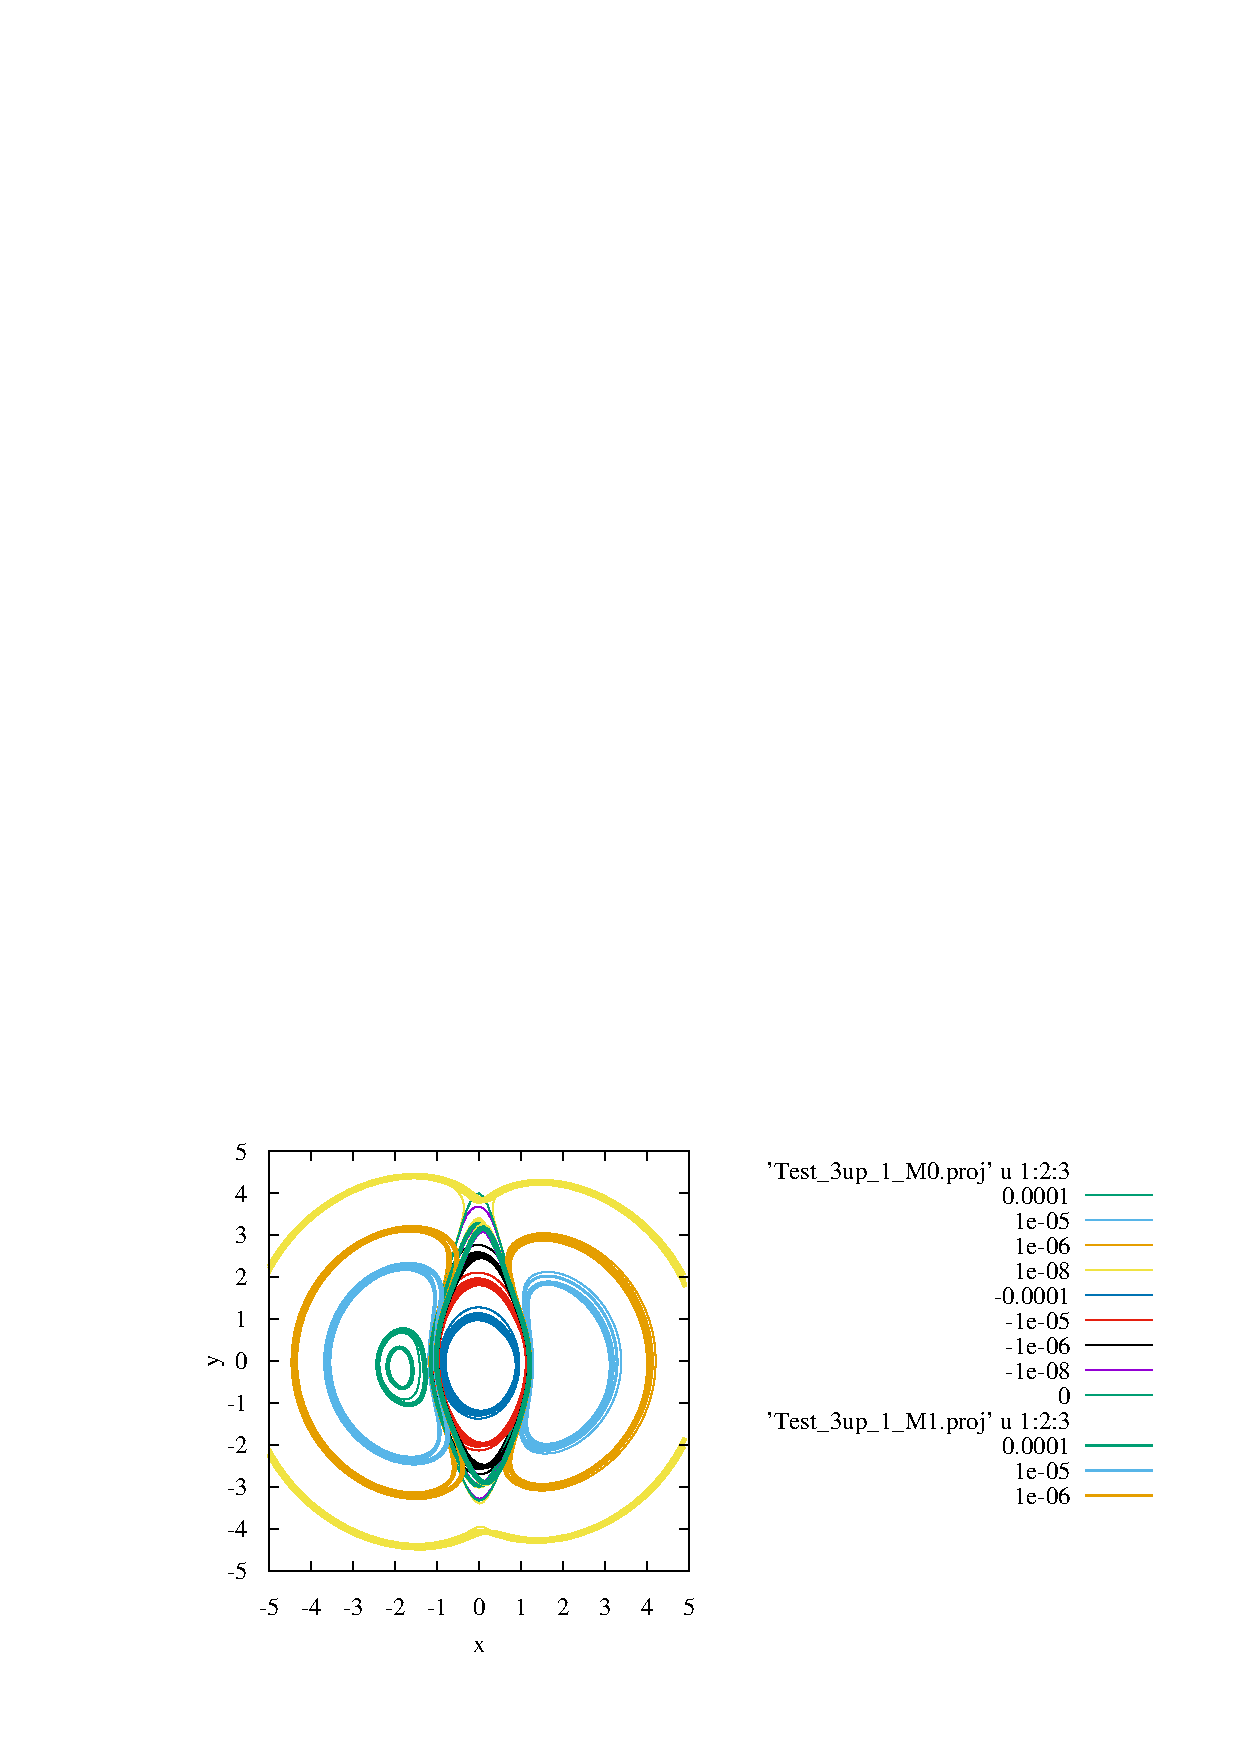
\includegraphics{Test_3up_1=1}%
\caption{\label{}}
\end{figure}

% Surround figure environment with turnpage environment for landscape
% figure
% \begin{turnpage}
% \begin{figure}
% \includegraphics{}%
% \caption{\label{}}
% \end{figure}
% \end{turnpage}

% tables should appear as floats within the text
%
% Here is an example of the general form of a table:
% Fill in the caption in the braces of the \caption{} command. Put the label
% that you will use with \ref{} command in the braces of the \label{} command.
% Insert the column specifiers (l, r, c, d, etc.) in the empty braces of the
% \begin{tabular}{} command.
% The ruledtabular enviroment adds doubled rules to table and sets a
% reasonable default table settings.
% Use the table* environment to get a full-width table in two-column
% Add \usepackage{longtable} and the longtable (or longtable*}
% environment for nicely formatted long tables. Or use the the [H]
% placement option to break a long table (with less control than
% in longtable).
% \begin{table}%[H] add [H] placement to break table across pages
% \caption{\label{}}
% \begin{ruledtabular}
% \begin{tabular}{}
% Lines of table here ending with \\
% \end{tabular}
% \end{ruledtabular}
% \end{table}

% Surround table environment with turnpage environment for landscape
% table
% \begin{turnpage}
% \begin{table}
% \caption{\label{}}
% \begin{ruledtabular}
% \begin{tabular}{}
% \end{tabular}
% \end{ruledtabular}
% \end{table}
% \end{turnpage}

% Specify following sections are appendices. Use \appendix* if there
% only one appendix.
%\appendix
%\section{}

% If you have acknowledgments, this puts in the proper section head.
%\begin{acknowledgments}
% put your acknowledgments here.
%\end{acknowledgments}

% Create the reference section using BibTeX:
\bibliography{pppNotes}

\end{document}
%
% ****** End of file apstemplate.tex ******

%
% \begin{table}%[H] add [H] placement to break table across pages
% \caption{\label{tab:compare} Cohesive energy of Si obtained through various computational methods and compared with experimental values.}
% \begin{ruledtabular}
% \begin{tabular}{l | c c c c}
% Method & DFT & VMC & DMC & Experiment \\
% \hline
% Energy (\electronvolt) & 5.28\footnotemark[1] & 4.48(1)\footnotemark[2] & 4.63(2)\footnotemark[2] & 4.62(8)\footnotemark[1] \\
% \end{tabular}
% \end{ruledtabular}
% \footnotetext[1]{Farid and Needs}
% \footnotetext[2]{Leung \emph{et~al.}}
% \end{table}
